\chapter{Track reconstruction with Graph Neural Networks}
\label{chap:graph-construction}

% The Combinatorial Kalman Filter (CKF) builds a track candidate locally, by incorporating clusters in the next layer which are compatible to an existing track state. 

Graph Neural Networks (GNNs) were first proposed in 2018 as an alternative track finder to the Combinatorial Kalman Filter (CKF)~\cite{farrell2018noveldeeplearningmethods}.
Developed and tested on the \textsc{TrackML} dataset \cite{trackml-particle-identification}, they demonstrated excellent physics performance and favourable scaling behaviour~\cite{exatrkx, choma2020trackseedinglabellingembeddedspace}.
Fundamentally, GNN-based algorithms represent a shift from the local track finding approach of the CKF to a global approach.
Instead of sequentially extending a tracklet\footnote{An incomplete track} with compatible hits on its path, as described in chapter \ref{chap:atlas-reco-chain}, global track finding considers simultaneously all connections between detector hits and finds those that are most likely to belong to true particle tracks.
No longer is a need to loop through a set of redundant track seeds, which makes the CKF slow and requires a costly ambiguity resolution.
The GNN ``looks at" all possible candidate tracks in an event at the same time, significantly accelerating the recognition of track patterns thanks to GPU-powered parallelization.
The shift from hit finding to connection finding necessitates a change in representation of the collision event from a point cloud to a collection of nodes and edges, the very definition of a \textbf{graph}. 
This approach therefore relies on graph data structure.

The work documented in this thesis builds upon that of reference \cite{exatrkx}, which examined the physics and computing performance of the GNN on the TrackML dataset~\cite{trackml-particle-identification}, and of reference \cite{Caillou:ATL-ITK-PROC-2022-006}, which made initial strides in applying the GNN to data from full ITk simulation. 
It contributes numerous developments that bring the new approach closer to the state-of-the-art performance.
Neural network architectures undergo significant refinements.
The algorithm is fully integrated into the official ATLAS analysis software framework~\cite{atlas_collaboration_2021_4772550}, thus enabling direct performance comparison to the CKF.
Finally, many components are computationally optimized, resulting in competitive reconstruction speed.
This chapter commence the discussion with an overview of the algorithm and the construction of graphs from detector data. 
Subsequent stages of the algorithm, especially the graph neural network, are detailed in chapters \ref{chap:gnn} and \ref{chap:track-building}, and finally the results are presented in chapters \ref{chap:tracking-performance} and \ref{chap:computing-performace}.
% In the previous chapter, we propose a global approach to the problem of track finding in the ITk as an alternative to the existing local approach of the Combinatorial Kalman Filter. 


\section{Overview}

The GNN-based approach, illustrated in figure \ref{fig:gnn4itk} and hereafter referred to as the \textbf{GNN4ITk} algorithm, creates track candidates by segmenting a graph constructed from the collection of space points in each event. 
A graph $G(V,E)$ is a mathematical structure consisting of a set of nodes $V$, and a set of pairwise connections $E$ between these nodes. 
Each node $v_i \in V$ represents a space point, and an edge $e_{ij} \in E$ a hypothesis that the space points represented by $v_i$ and $v_j$ are created from successive energy deposits by the same particle. 
In addition, a ground truth graph $G_{truth}= (V, E_{truth})$ is defined from the same set $V$ and the connections between successive space points on the trajectories of all particles in the event, denoted by $E_{truth}$, oriented in the direction of increasing distance from the particle's production vertex. 
An edge $e_{ij}\in E$ is true if it is also in the truth graph, i.e. 
\begin{equation}
\label{eq:9.1}
y_{ij} = 1_{[e_{ij} \in E_{truth}]},
\end{equation}
and fake otherwise. 
A graph neural network is used to assign to every edge $e_{ij} $ a score $s_{ij} = P[y_{ij} = 1]$, representing a continuous function of the probability that the edge in question is true.
To obtain the probability, a calibration step is sometimes needed \cite{Feng_2022}. 
For our purpose, a score threshold is selected to satisfy certain requirements on the edge efficiency evaluated on the validation set.
Edges with scores under the threshold are eliminated, and the remaining graph is segmented into \textbf{track candidates}, collections of nodes believed to originate from the same particle.

\begin{figure}[h!]
    \centering
    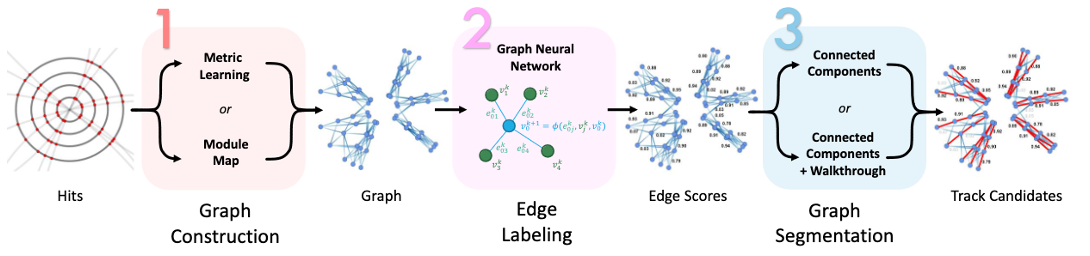
\includegraphics[width=\textwidth]{figures/gnn4itk.png}
    \caption{The GNN4ITk algorithm consists of three distinct stages. The first stage constructs a graph from the set of space points in an event, each acting as a node. The second stage identifies edges connecting consecutive nodes on a particle tracks from other edges. The last stage construct track candidates by segmenting the graph using the output of the second stage. The algorithm's output consists of individual track candidates each as a set of space points believed to belong to the same particle.}
    \label{fig:gnn4itk}
\end{figure}

\section{Target, non-target particles and evaluation metrics}
\label{sect:eval-metrics}
At $\epu=200$, each collision event produces $\expval{N}\approx 10000$ particles, the majority of which are of little interest to the physics program in ATLAS. 
They include, for example, low-momentum particles from background processes or particles which leave too few hits to be considered reconstructible.
The remaining particles can be broadly categorized by the interaction from which they emerge. 
Primary particles are produced in the luminous area directly from proton-proton interaction and stable enough to traverse the detector, including protons, electrons, muons, pions, etc.
Secondary particles arise from the interaction of primary particles with detector material, such as $\delta$-ray electrons and nuclear interaction products. 
As these interactions destroy information on the primary particle's kinematics, the CKF chain does not target secondary particles for reconstruction.
In the same spirit, throughout the GNN4ITk chain, we identify these particles prior to model training and exclude them from the loss function, as well as performance evaluation.

Since a secondary interactions occurs when the primary particle has travelled a distance from the luminous region, their vertices are considerably further from the origin than the primary counterpart. 
Shown on figure \ref{fig:vertex-spectrum}, the majority of primary vertex positions are located at $v_r < 20$ cm and $v_z < 20$ cm, in contrast to secondary vertices, whose distributions of $v_r$ and $v_z$ are more spread-out and with longer tails.
% for secondary particles than their primary counterpart, which terminates at $v_r<10$ cm and $\abs{v_z}< 20$ cm, see figure \ref{subfig:radius-spectrum}.
This distinction allows us to select primary particles in training by requiring the production vertex to be within 26 cm from the origin.
As we will see in chapter \ref{chap:tracking-performance}, the ATLAS reconstruction chain eliminates secondary particle tracks by applying selection cuts on the impact parameters, which are good estimates of the vertex point, of $\abs{z_0}\le 20$ cm and $\abs{d_0}\le10$ cm. 

\begin{figure}[h!]
\begin{subfigure}[b]{0.49\textwidth}
    \centering
    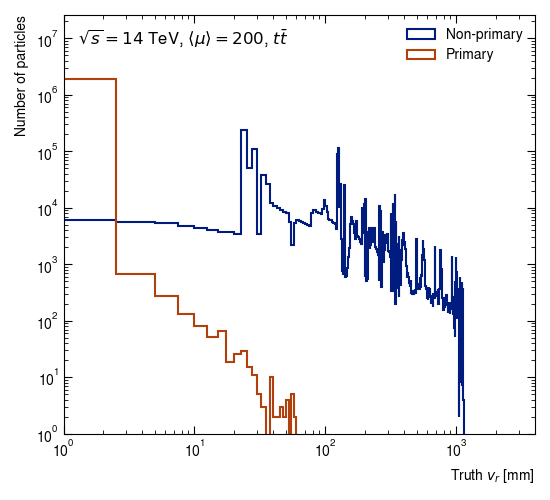
\includegraphics[width=\textwidth]{figures/vr-hist.png}
    \caption{}
    \label{subfig:radius-spectrum}
\end{subfigure}
\begin{subfigure}[b]{0.49\textwidth}
    \centering
    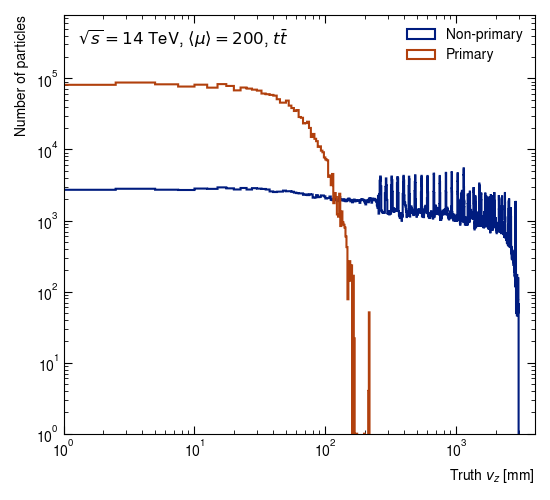
\includegraphics[width=\textwidth]{figures/vz-hist.png}
    \caption{}
    \label{subfig:z-spectrum}
\end{subfigure}
    \caption{Distributions of the production vertex position on the transverse plane (a) and along the $z$-axis (b) of simulated particles in $t\bar{t}$-events at $\epu=200$ for non-primary and primary particles. Primary vertices are restricted to a small region around the interaction point, whereas non-primary vertices can occur throughout the detector.}
    \label{fig:vertex-spectrum}
\end{figure}

As we have seen in section \ref{subsect:e-loss-electron}, electrons and positrons uniquely undergo significant energy loss due to Bremsstrahlung, and often follow trajectories that deviate from a helix. 
To guarantee good electron efficiency without compromising that of other particles, the ATLAS chain reconstructs electron tracks in a separate pass with a specialized parameter estimation technique. 
Similarly, we avoid training models on ``irregular" electron tracks by excluding their contribution from the loss function.

Because each simulated event is generated from one hard-scattering (HS) collision and on average 200 pile-up collisions (section \ref{sect:simulated-samples}), particles originating from soft interactions outnumber HS particles by about two orders of magnitude, (figure \ref{subfig:eta-spectrum}). 
HS particles are generally more energetic; their $\pT$ spectrum stretches up to 100 GeV, whereas that of pile-up particles strongly peaks at $\pT<1$ GeV and terminates at 20 GeV, as shown in figure \ref{subfig:pt-spectrum}. 
% widely differ, with the former having a much longer tail.
As a consequence, a loss function calculated from all edges in the event is dominated by examples from low-$\pT$ tracks and bias the model toward pile-up particles, at the expense of high-$\pT$ HS particles that represent the interesting physics.
This data imbalance largely impacts the performance, since in the presence of the magnetic field, low-$\pT$ particles have larger curvature and therefore different track pattern than do high-$\pT$ particles.
To cope with this problem, we neglect the contribution to the loss function from particles of $\pT<1$ GeV.

\begin{figure}[h!]
\begin{subfigure}[b]{0.49\textwidth}
    \centering
    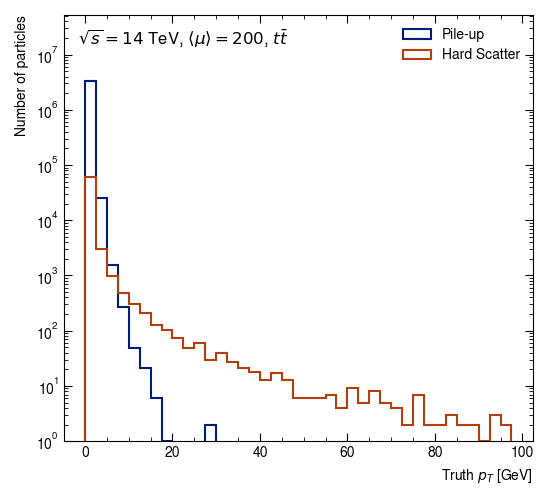
\includegraphics[width=\textwidth]{figures/pt-hist.png}
    \caption{}
    \label{subfig:pt-spectrum}
\end{subfigure}
\begin{subfigure}[b]{0.49\textwidth}
    \centering
    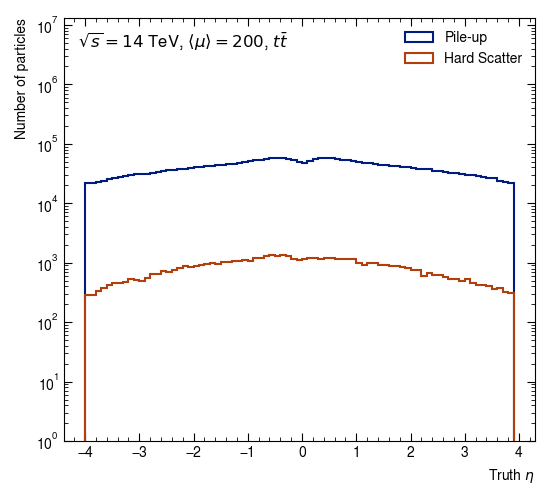
\includegraphics[width=\textwidth]{figures/eta-hist.png}
    \caption{}
    \label{subfig:eta-spectrum}
\end{subfigure}
    \caption{Distributions of transverse momentum \pT (a) and pseudorapidity (b) of simulated particles in $t\bar{t}$-events at $\epu=200$ separated according into hard-scattering and pile-up particles. Soft pile-up particles have low \pT, whereas hard-scattering particles have a wider \pT distribution. The former is two orders of magnitude more abundant than the latter.}
    \label{fig:pt-eta-spectrum}
\end{figure}

In light of this discussion, we sort truth particles into two subsets by the following criteria
\begin{enumerate}
    \item \textbf{Target} particles: primary particles from both hard-scattering and pile-up interactions, which have $\pT>1$ GeV and $\abs{\eta}<4$, leave at least 3 hits in the tracker, are produced at a transverse radius $R<26$ cm, and are not electron nor positrons.
    \item \textbf{Non-target} particles: The rest of truth particles, including electrons and other particles not satisfying the kinematic selection.
\end{enumerate}
In the same manner, the subset of $E_{truth}$ comprising exclusively connections from target particles is called the target truth edges and denoted as $E_{truth,target}$. 
A subset of non-target truth edges is defined as $E_{truth, non-target} = E_{truth} - E_{truth,target}$. 
The objective of global track finding then is to identify as many target truth edges and to misidentify as few fake edges as possible.
Two metrics are defined from the edge sets to quantify these criteria.
The first is the \textbf{edge efficiency} $\epsilon$: the fraction of target true edges present in a given edge set $E$
\begin{equation}
\label{eq:9.2}
\epsilon = \frac{\abs{E \cap E_{truth,target}  }} {\abs{E_{truth, target}}},
\end{equation}
and the second is the \textbf{edge purity} $\rho$: the fraction of target true edges in $E$, excluding non-target true edges
\begin{equation}
\label{eq:9.3}
\rho = \frac{\abs{E_{truth,target} \cap E  }} {\abs{ E - E_{truth, non-target} } } .
\end{equation}
% These definitions ensure that non-target particles do not contribute to model performance. 
High edge efficiency indicates that $E$ contains a large proportion of target edges in the event, while high purity means that a small proportion of $E$ is fake edges.
These definitions also explicitly exclude non-target particles from the evaluation of model performance.

\section{Graph construction methods}
\label{sect:graph-construction}
The first step of the GNN4ITk chain constructs a graph from the collision event. 
After the space point formation stage, discussed in section \ref{sect:cluster-spacepoint}, an event is a set of space points, which can be considered as a graph with an empty edge set $G_0=(V, E=\varnothing)$. 
The graph construction stage populates $E$ with edges, with an objective of including as many target edges as possible, and at the same time control the total number of edges such that the resulting graph can fit on GPU memory to train the GNN. 
At $\epu=200$, a $t\bar{t}$ event has $\mathcal{O}(10^5)$ space points, and a fully-connected graph, though simple, would have $\mathcal{O}(10^{10})$ edges, most of which are unphysical and a too expensive to process.
Such a sizeable graph would also be unable to fit on the GPU memory. 
Therefore, more clever methods are needed to construct the graph. 
We investigate two graph construction methods: Module Map and Metric Learning. 

\subsection{The Module Map Method}
\label{subsect:module-map}

The module map is a data-driven approach to construct a graph. 
It is based on the observation that a small fraction of edges in a fully-connected graph is physical, and an even smaller fraction comes from target particles.
It is therefore possible to create a list of all pairs of detector modules connected by target particles in a large number of $t\bar{t}$ events. 
By following the path of each target particle and recording pairs of modules that it sequentially traverses, we build up this list and call it the \textbf{Module Map}. 
To maximize the coverage of possible module connections, 90000 $t\bar{t}$ simulated events described in section \ref{sect:simulated-samples} are used

Illustrated in figure \ref{fig:module-map} is an example of module map learning, in which two particles are observed to sequentially hit modules $1\rightarrow2\rightarrow 3 \rightarrow 4 \rightarrow 5 \rightarrow 6$ and $3\rightarrow 4 \rightarrow 7 \rightarrow 8 \rightarrow 9$. 
From these particles, connections between the following pairs of modules (1,2), (2,3), (3,4), \textbf{(4,5)}, (5,6), \textbf{(4,7)}, (7,8), and (8,9) are registered to the module map (note the presence of two connections sharing module number \textbf{4}). 
As more particles are observed, the set of recorded connections grows, covering a wider range of module connectivity.
The idea is that once the number of observed events is large enough, the map is saturated and becomes a ``dictionary" of all possible module connections.

\begin{figure}[h!]
    \centering
    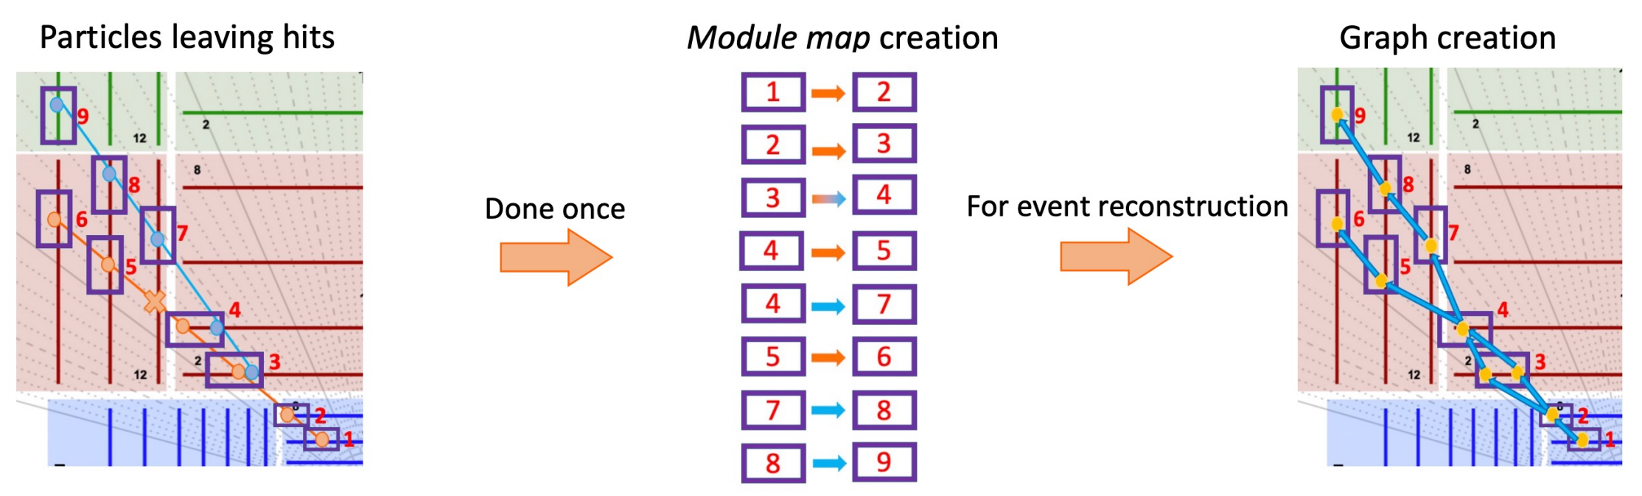
\includegraphics[width=1\linewidth]{figures/module-map.png}
    \caption{Principle of the Module Map method for graph construction.  By observing the trajectory of target particles in 90000 $t\bar{t}$ events, a list of all pairs of detector modules sequentially traversed by a particle is built. During event reconstruction, the space points residing on the pairs of modules which appear in the module map are connected by an edge. A set of selections are applied to reduce the number of edges and eliminate outliers.}
    \label{fig:module-map}
\end{figure}

When building a graph from an event \textit{which has not been seen} by the Module Map, out of all possible connections between space points, only those linking pairs of modules present in the Module Map are admitted to become graph edges. 
On figure \ref{fig:module-map}, for example, 10 space points on 9 modules are recorded in the new event, with 2 space points present on module 3. 
The module map therefore admits connections between space points residing on the following module pairs: (1,2), $(2,3_1)$, $(2,3_2)$, $(3_1,4)$, $(3_2,4)$, (4,5), (4,7), (5,6), (7,8), (8,9), with subscripts indicating different space points on the same module where necessary. 
The module map thus allows to select a small subset of the 90 possible connections, based on our previous observations. 

The same principle can be extended from pairs of modules to triplets of modules, so that the module map is built from a list of three modules sequentially hit by a particle, and on inference, pairs of possible connections appearing in the module map are admitted. 
Since the requirement of three consecutive hits is stricter than that on two hits, the \textit{triplet} module map helps reduce the number of edges in the reconstructed graph compared to the simple \textit{doublet} module map. 
Nevertheless, the average number of edges in graphs constructed from the triplet module map is still too large to process on available hardware, averaging $\mathcal{O}(10^8)$. 

On the chosen GNN architecture, we found that a GPU with 80GB memory is capable of running the forward pass with gradient tracking on $\sim 2\times 10^6$ edges/graph, which is the target of graph construction. 
The number of edges per event acts as a batch size which can limit the number of trainable parameters in a neural network and its expressive power.
% In addition, the number of target edges per event is of $\mathcal{O}(10^4)$, a graph of $\mathcal{O}(10^8)$ edges contains far more fake than true edges and creates a severe class imbalance.
In addition, processing a massive graph of mostly fake edges is a computing a bottleneck. 
To build leaner graphs, additional selection requirements are imposed on doublets and triplets in the ``crude" module map graphs.

Edge selections are based on geometric features derived from the connected space points. 
Denoting the nodes in a doublet ordered by increasing distance from the origin by $(v_1, v_2)$, and in a triplet in the same order by $(v_1, v_2, v_3)$, we define two categories of geometric features.
\begin{enumerate}
    \item \textbf{Doublet features} are calculated from the doublet hits connected by an edge. They include:
    \begin{itemize}
        \item $z_0 = z_1-r_1\frac{z_2-z_2}{r_2-r_1}$.
        \item $\Delta\phi=\phi_2-\phi_1$
        \item $\Delta\eta = \eta_2-\eta_1$
        \item $\phi_{slope}=\frac{\phi_2-\phi_1}{r_2-r_1}$.
    \end{itemize}
    These features represent several basic assumptions about the trajectory of a charged particle in a magnetic field. 
    For example, the pseudorapidity $\eta$ depends only on the polar angle $\theta$ and is constant if the particle does not interact with materials. 
    The distribution of $\Delta \theta$ of two consecutive hits on a particle's path should therefore peak at $0$ with some width $\sigma$ resulting from detector effects. 
    \item \textbf{Triplet features} are calculated from the doublet features of the pair of edges, resembling a second-order derivative. 
    \begin{itemize}
        \item $\Delta\mathrm{slope}_{xy} = \left(\frac{\Delta y}{\Delta x}\right)_{12}$ - $\left(\frac{\Delta y}{\Delta x}\right)_{23}$
        \item $\Delta\mathrm{slope}_{rz} = \left(\frac{\Delta z}{\Delta r}\right)_{12}$ - $\left(\frac{\Delta z}{\Delta r}\right)_{23}$
    \end{itemize}
    where $\Delta u$ is the difference in variable $u$ between the nodes indicated by the numerical subscript. $\Delta\mathrm{slope}_{xy}$ is related to the curvature of the orbit and $\Delta\mathrm{slope}_{rz}$ the deviation from a straight line over the two triplet connections.
\end{enumerate}
The empirical distributions of these features are established from events dedicated to the construction of the module map, along with a set of thresholds that defines the acceptance region. 
These thresholds are selected to eliminate as many fake edges as possible without rejecting true edges in the observed 90000 events. 
In inference, any edge failing to meet these thresholds is rejected. 
A simple choice for the acceptance region of a feature $\xi$ is the whole range $[\xi_{min}, \xi_{max}]$, such that an inferred edge is rejected if $\xi < \xi_{min}$ or $\xi>\xi_{max}$. 
This is called the \textbf{\textsc{MinMax}} selection. 
Another choice is the interval of $[\bar{\xi} - 5\sigma_{\xi}, \bar{\xi}+5\sigma_{\xi}]$, where $\bar{\xi}$ and $\sigma_{\xi}$ are respectively the sample mean and standard deviation of the feature, denoted the \textbf{\textsc{MeanRMS}} selection. 
Both selections are examined, and the graph construction result is discussed in section \ref{sect:graph-contruction-performance}.

\subsection{The Metric Learning approach}
\label{subsect:metric-learning}

Metric Learning~\cite{metric-learning-rev1, metric-learning-rev2, metric-learning-rev3} is a semi-supervised machine learning technique which models the difference between a pair of data points. 
Given a sample  $X$ and corresponding labels $Y$, we seek a transformation $f_{\theta}: \mathbb{R}^d\rightarrow \mathbb{R}^n$, where $d$ is the dimension of $\mathbf{x}\in X$, $n$ the dimension of an embedding space and $\theta$ a set of learnable weights. 
A distance metric $\mathcal{D}: \mathbb{R}^n \otimes \mathbb{R}^n \rightarrow [0, \infty)$ is selected to measure the difference between two data points in the embedding space. 
The objective is that for two examples $\mathbf{x}_i, \mathbf{x}_j \in X$ and their labels $y_j, y_j\in Y$, the distance $ \mathcal{D}(f_{\theta}(\mathbf{x}_i), f_{\theta}(\mathbf{x}_j))$ is small if $y_i=y_j$ and large otherwise. 
After training, the transformation $f$ sends data points of the same class labels to the same region in the embedding space, and separate those having different labels (figure \ref{fig:metric-learning-illus}).
For conciseness, we define
% in this case a pair of nodes $(i,j)$ equipped with feature vectors $\mathbf{x}_i, \mathbf{x}_j \in \mathbb{R}^n$, via a metric function $\tilde{d}: \mathbb{R}^n \otimes \mathbb{R}^n \rightarrow [0, \infty)$. The metric function is of the form 
\begin{equation}
\label{eq:9.4}
d_{\theta}(\mathbf{x}_i, \mathbf{x}_j) = \mathcal{D}(f_{\theta}(\mathbf{x}_i), f_{\theta}(\mathbf{x}_j)), 
\end{equation} 
The distance metric can be any mapping that satisfies the following criteria, defined for all $\mathbf{z}_i, \mathbf{z}_j, \mathbf{z}_k \in \mathbb{R}^n $
\begin{enumerate}
    \item non-negativity: $\mathcal{D}(\mathbf{z}_i, \mathbf{z}_j) \ge 0 $
    \item symmetry: $\mathcal{D}(\mathbf{z}_i, \mathbf{z}_j) = \mathcal{D}(\mathbf{z}_j, \mathbf{z}_i)$ 
    \item identity: $\mathcal{D}(\mathbf{z}_i, \mathbf{z}_i) = 0$
    \item triangle inequality: $\mathcal{D}(\mathbf{z}_i, \mathbf{z}_j) \le \mathcal{D}(\mathbf{z}_i, \mathbf{z}_k) + \mathcal{D}(\mathbf{z}_k, \mathbf{z}_j)$
\end{enumerate}

To construct a graph using metric learning, we assume that two nodes belonging to different tracks differ from each other in some sense. 
Taking $X$ as the set of node feature vector, and $Y$ the set of the particle label, we can write $y_{ij} = 1_{[y_i=y_j]},\, y_i\in Y$.
Through metric learning, the transformation weights $\theta$ are adjusted to minimize $d_{\theta}(\mathbf{x}_i, \mathbf{x}_j)$ if $y_{ij}=1$ and maximize it if $y_{ij}=0$.

\begin{figure}[h!]
    \centering
    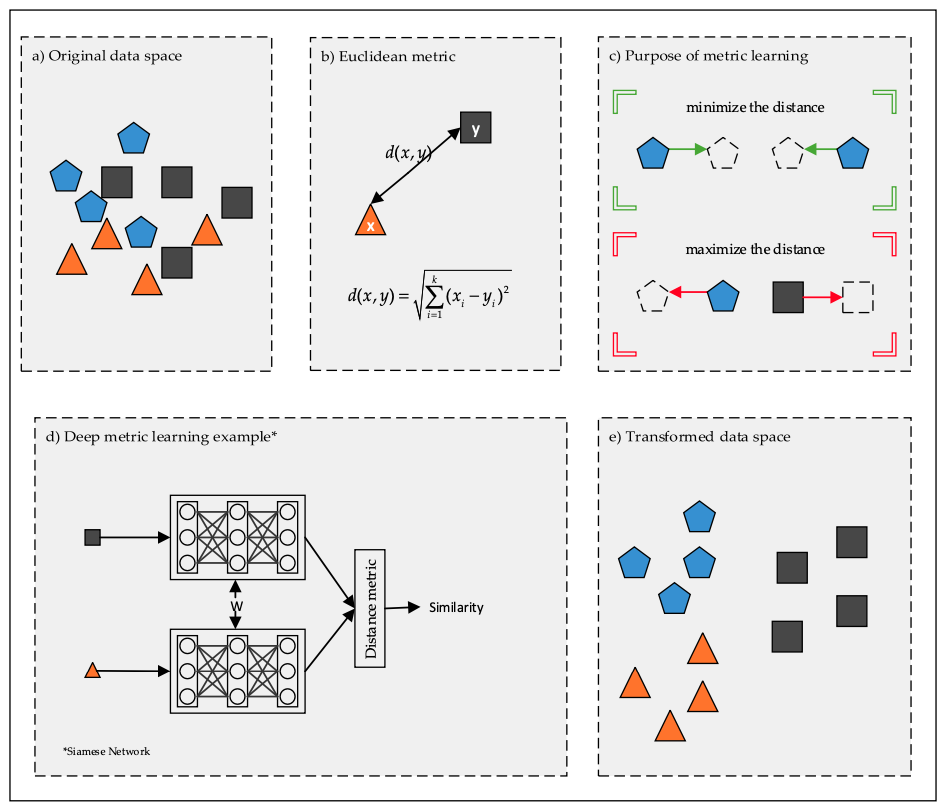
\includegraphics[width=0.8\textwidth]{figures/metric-learning-illustration.png}
    \caption{Principle of deep metric learning. Starting from (a) labelled data which are difficult to separate in real space, (b) a distance metric is defined to measure the similarity between data points in an embedding space, in this case a simple Euclidean distance. (c) A transformation from real to embedding space is learned, such that examples of the same class are close together, whereas those of different classes are pushed away from each other. (d) The transformation is a simple feed-forward network applied to to all instances of the dataset. (e) After training, examples of different classes are well-separated, and clusterizable \cite{metric-learning-rev2}.}
    \label{fig:metric-learning-illus}
\end{figure}

The Euclidean distance is chosen as distance metric
\begin{equation}
    \mathcal{D}(\mathbf{p},\mathbf{q}) = \Vert \mathbf{p} - \mathbf{q} \Vert_2 = \sqrt{ (\mathbf{p} - \mathbf{q})^2 }, \quad \mathbf{p}, \mathbf{q}\in \mathbb{R}^n,
\end{equation}
and a simple Multi-Layer Perceptron (MLP) as the transformation $f_{\theta}$. The last ingredient is the loss function $\mathcal{L}(\theta)$. There are many choices of loss function for metric learning, each targeting a slightly different learning objective. A comprehensive summary is given in references \cite{metric-learning-rev2, metric-learning-rev4}. In this thesis, the simplest and most intuitive choice, called \textbf{Contrastive Loss}, is employed. Over a set of edges $E$, we define
\begin{equation}
    \label{eq:9.6}
    \mathcal{L}_{E}(\theta) = \frac{1}{\abs{E}} \sum_{e_{ij}\in E} l_{\theta}(\mathbf{x}_i, \mathbf{x}_j), \quad l_{\theta}(\mathbf{x}_i, \mathbf{x}_j) = y_{ij}d_{\theta}(\mathbf{x}_i, \mathbf{x}_j) + (1-y_{ij})\max\{0, r-{d_{\theta}}(\mathbf{x}_i, \mathbf{x}_j) \}.
\end{equation}
For a positive pair $(y_{ij}=1)$, the loss function is minimized if the distance between $f_{\theta}(\mathbf{x}_i)$ and $f_{\theta}(\mathbf{x}_j)$ is 0, effectively pulling together $(\mathbf{x}_i, \mathbf{x}_j)$.
For a negative pair $(y_{ij}=0)$, the loss is minimized if their distance is increased up to a margin $r$. 
$l_{\theta}(\mathbf{x}_i, \mathbf{x}_j)$ becomes 0 if $d_{\theta} > r$. 
This margin prevents the model from enlarging the distance when the pair of nodes is sufficiently separated, focusing the attention on those that are not. 
The contrastive loss defined with a margin is also called the contrastive hinge loss. 
% Assuming $E$ contains both true and fake edges, optimizing $L(E)$ is tantamount to finding a transformation $f$ that minimizes $\abs{f(\mathbf{x}_i) - f(\mathbf{x}_j)}$ if $e_{ij}$ is a target true edge $(e_{ij} \in E_{truth,target})$ and maximising it to at least a distance $r$ if $e_{ij}$ is fake $(e_{ij} \notin E_{truth})$. 

Note that the loss is computed from pairs of nodes, which can be regarded as edges, but we do not have edges at this point. 
A training sample $E$ must therefore be generated from the input nodes. 
Again, a simple choice of all $N(N-1)$ possible unordered pairs of node is far too many to fit on memory and would overwhelmingly contain fake edges. 
Instead, we construct $E$ using a technique called hard negative mining \cite{robinson2021contrastivelearninghardnegative}
\begin{equation}
    \label{eq:9.7}
    {E} = E_{truth, target} \cup E_{hnm} \cup E_{random},
\end{equation}
where $E_{truth, target}$ is the set of target true edges as defined in \ref{sect:eval-metrics}. 
This is truth information that comes from the training data. 
To generate training fake edges, a training graph is constructed in the latent space by connecting each node $v_i \in V$ to a maximum of $k$ closest nodes within a sphere centered at $v_i$ of radius $r$ using a k-Nearest-Neighbor algorithm (kNN). 
Note that the radius is equal to the margin. 
A set of edges, denoted $E_{hnm}$, is constructed from the training graph by finding $n_{hnm}$ fake edges with the smallest distance in the transformed space.
$E_{hnm}$ represents the negative pairs that most resemble true pairs, so maximizing their distance is equivalent to lower-bounding the separation between all fake pairs of nodes. 
Finally, a set of randomly sampled edges $E_{random}$ is added to stabilise the loss. %The graph is constructed in the latent space by connecting each node $v_i \in V$ to a maximum of $k$ closest nodes within a sphere centered at $v_i$ of radius $r$ using a k-Nearest-Neighbor algorithm (kNN).

\newpage
\begin{table}[h!]
    \centering
    \begin{tabular}{l|l}
    \hline
     Hit input    &  Description\\
     \hline
      $r$   & Global transverse radius of space point \\
      $\phi$ & Global azimuthal angle of space point\\
      $z$ & Global $z$-coordinate of space point\\
      $x_{CL, i}$ & Global $x$-coordinate of cluster $i$ \\
      $y_{CL, i}$ & Global $y$-coordinate of cluster $i$ \\
      $z_{CL, i}$ & Global $z$-coordinate of cluster $i$ \\
      count & Number of pixels cells contained in a cluster \\
      charge count & Charge deposit on a pixel cluster \\
      $\eta_{CL,loc,i}$ & Module $\eta$ in local coordinate system \\
      $\phi_{CL,loc,i}$ & Module $\phi$ in local coordinate system \\
      $\eta_{CL,glob,i}$ & Module $\eta$ in global coordinate system \\
      $\phi_{CL,glob,i}$ & Module $\phi$ in global coordinate system \\
      eta-angle & hit $\eta$ angle \\
      phi-angle & hit $\phi$ angle \\
      $l_x$ (LocalDirx) & Cluster shape $x$\\
      $l_y$ (LocalDiry)& Cluster shape $y$\\
      $l_z$ (LocalDirz)& Cluster shape $z$\\
      LengthDirx & LengthDirx \\
      LengthDiry & LengthDiry \\
      LengthDirz & LengthDirz \\
      \hline
    \end{tabular}
    \caption{Input features into the Metric Learning model. See Appendix \ref{appendix:hit-training-var} for definitions of the variables.}
    \label{tab:input-metric-learning}
\end{table}

\begin{table}[h!]
    \centering
    \begin{tabular}{l|l}
    \hline
      Hyperparameter   &  Value \\ \hline 
       Hidden layers   & 4\\
       Hidden dimension& 1024 \\
       Embedding dimension & 12 \\
       KNN & 50 \\
       Margin & 0.1 \\
       Weighting ratio & $1.0:4.0$ \\
    \hline
    \end{tabular}
    \caption{Hyperparameters used to train the Metric Learning model.}
    \label{tab:metric-learning-specification}
\end{table}

\newpage

% \begin{figure}[h!]
%     \centering
%     
\includegraphics[width=0.9\textwidth]{figures/placeholder.jpeg}
%     \caption{Metric Learning training curves}
%     \label{fig:metric-learning-training-curve}
% \end{figure}

The model was trained on an NVIDIA A100 GPU with 80 GB in memory. 
The train set contains 7800 simulated $t\bar{t}$ events, each treated as a batch. 
An iteration over the train set (epoch) takes approximately 1 hour, and the model is trained over approximately 200 epochs. 
% Shown in figure \ref{fig:metric-learning-training-curve} are the training curves (fill in discussion on training)

\section{Result}
\label{sect:graph-contruction-performance}

Shown in figure \ref{fig:mm-eff} is the averaged edge efficiency of graphs constructed with the \textbf{\textsc{MinMax}} and \textbf{\textsc{MeanRMS}} selections as a function of the pseudorapidity $\eta$\footnote{Here the pseudorapidity of an edge is defined as that of the inner node.} and transverse momentum $\pT$. 
The Module Map method under both choices of edge cuts produces efficiency $\epsilon\ge 99.5\%$ across $\eta$. 
Averaged across test events, the \textbf{\textsc{MeanRMS}} selection is slightly less efficient than the \textbf{\textsc{MinMax}} counterpart by $0.2\%$, due to tighter thresholds on geometric observables. 
The former's inefficiency is observed in the barrel region $(\abs{\eta}<2)$ and the very forward region $(\abs{\eta} \approx 4)$.
The slight efficiency loss comes with the benefit of building smaller graphs.
The \textbf{\textsc{MeanRMS}} selection produces graphs having $\expval{|V|} = (8.55\pm2.26)\times10^5$ edges, $30\%$ fewer than those from the latter, averaging at $(1.22\pm0.31)\times10^6$ edges.

\begin{figure}[h!]
\begin{subfigure}[b]{0.49\textwidth}
    \centering
    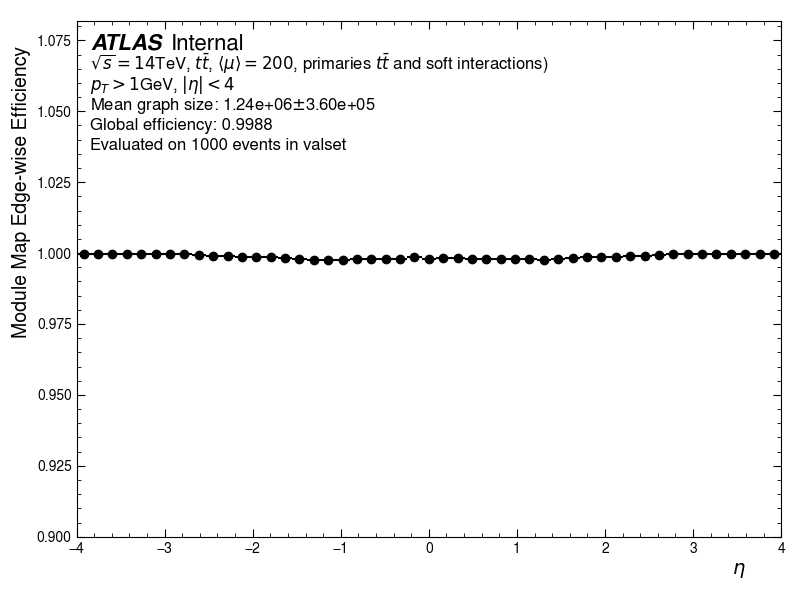
\includegraphics[width=\textwidth]{figures/gnn_MM_UNCLEANED_MINMAX_WITHOUT_CONCAT_LATENT128_LN/graph_construction_edgewise_efficiency_eta.png}
    \caption{}
    \label{subfig:mm-eff-minmax-eta}
\end{subfigure}
\begin{subfigure}[b]{0.49\textwidth}
    \centering
    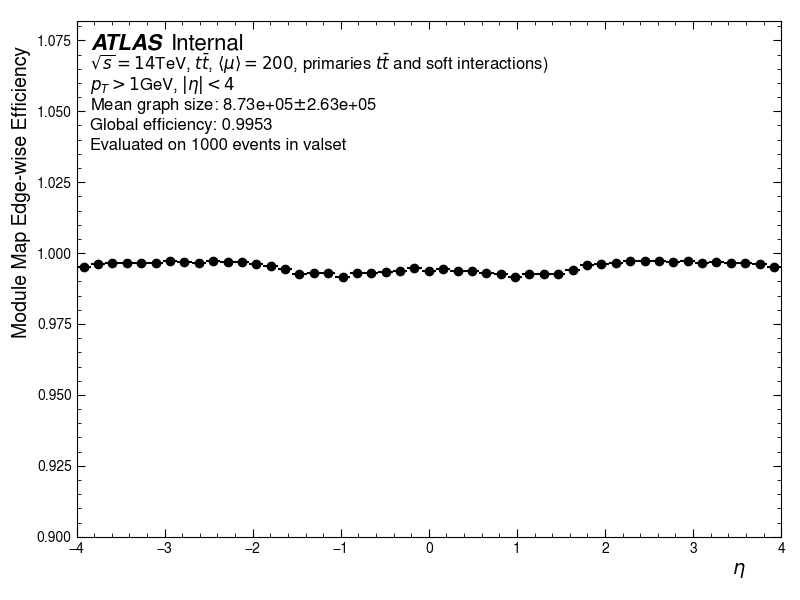
\includegraphics[width=\textwidth]{figures/gnn_MM_UNCLEANED_MEANRMS_WITHOUT_CONCAT_LATENT128_LN/graph_construction_edgewise_efficiency_eta.png}
    \caption{}
    \label{subfig:mm-eff-meanrms-eta}
\end{subfigure}

\begin{subfigure}[b]{0.49\textwidth}
    \centering
    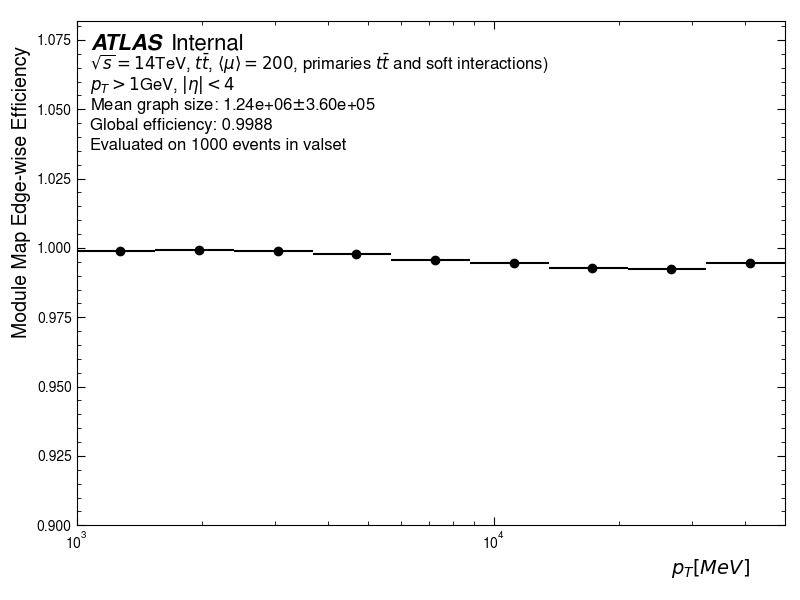
\includegraphics[width=\textwidth]{figures/gnn_MM_UNCLEANED_MINMAX_WITHOUT_CONCAT_LATENT128_LN/graph_construction_edgewise_efficiency_pt.png}
    \caption{}
    \label{subfig:mm-eff-minmax-pt}
\end{subfigure}
\begin{subfigure}[b]{0.49\textwidth}
    \centering
    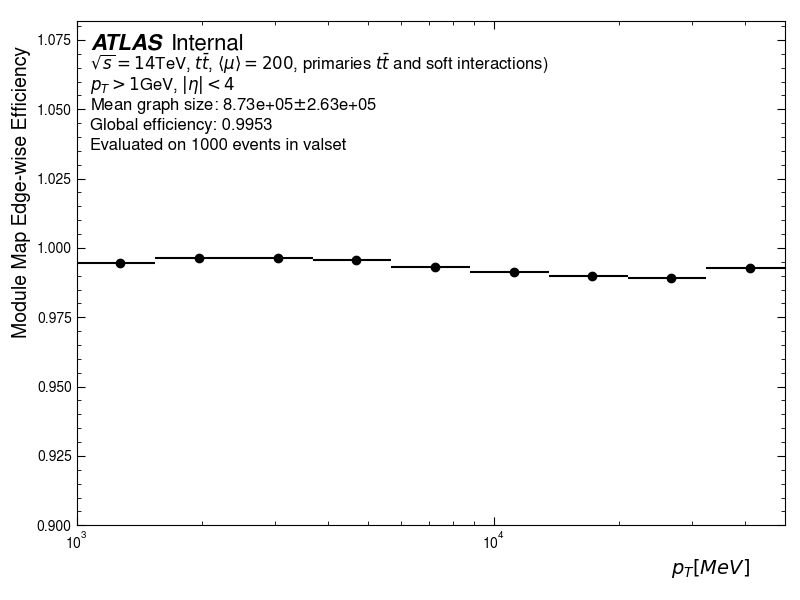
\includegraphics[width=\textwidth]{figures/gnn_MM_UNCLEANED_MEANRMS_WITHOUT_CONCAT_LATENT128_LN/graph_construction_edgewise_efficiency_pt.png}
    \caption{}
    \label{subfig:mm-eff-meanrms-pt}
\end{subfigure}
    \caption{Graph construction efficiency of the Module Map approach as a function of $\eta$ (upper) and $\pT$ (lower), using the MinMax selection (left) and MeanRMS selection (right). }
    \label{fig:mm-eff}
\end{figure}

The reduced number of edges at negligible efficiency cost is a strong advantage of the \textbf{\textsc{MeanRMS}} method. 
It allows the GNN to be trained with better class balance, because the majority of additional eliminated edges are fake or non-target, evidenced by almost identical efficiency values. 
In addition, a smaller graph leads to better latency and smaller memory footprint, which are important factors in inference. 
Therefore, graphs produced by both selections are examined in later stages of the reconstruction chain.

Both of the module map selections show good edge efficiency over the $\pT$ range, reaching $\epsilon \ge 99\%$ (figures \ref{subfig:mm-eff-minmax-pt} and \ref{subfig:mm-eff-meanrms-pt}).
A slight decrease is observed at the high-$\pT$ region, above $\pT \ge 5$ GeV, which, as we will see in the next chapters, is a common occurrence in the GNN4ITk chain.
% As we will see in subsequent chapters, this inefficiency at high-$\pT$ is a common occurrence in the GNN4ITk chain. 
It can be attributed to the rarity of high-$\pT$ particles in the training data, as discussed in section \ref{sect:eval-metrics}, which affects the coverage of possible module connections produced by high-$\pT$ particles.
% Even though it does not ``learn" to recognize patterns in machine learning argot, the module map memorizes the module connections in the training events, and reproduces them in an inference event. 
The Module Map can only create an edge in the inferred event if it has seen the same edge during its construction
In other words, in order for a true connection to appear in the inferred graph, the corresponding pair of modules must have been consecutively traversed by a particle in the training events.
However, high-$\pT$ particles constitute but a small portion of final-state particles (figure \ref{subfig:pt-spectrum}), and those observed from the training event might not cover all possible trajectories through the detector's modules.
As a result, it is more likely that a high-$\pT$ connection from a target particle in an inferred event was not seen in the training events, leading to inefficiency.

\begin{figure}[h!]
\begin{subfigure}[b]{0.49\textwidth}
    \centering
    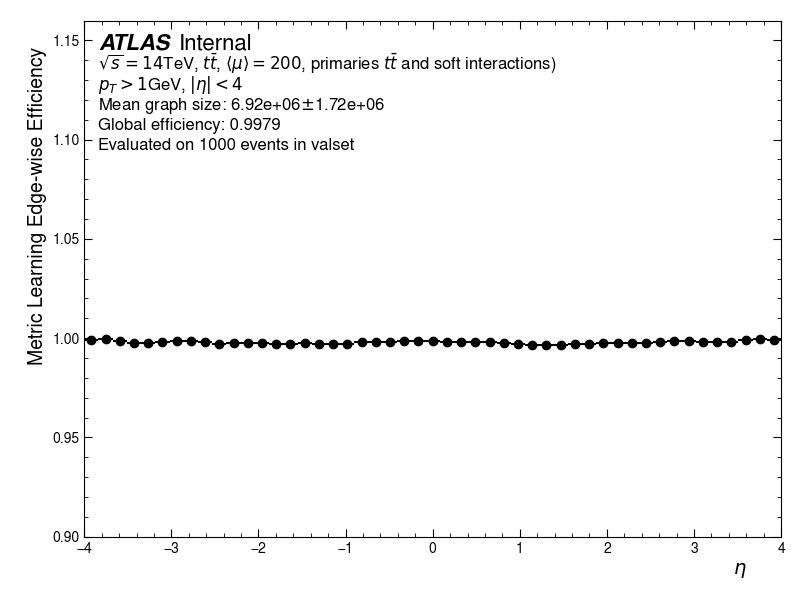
\includegraphics[width=\textwidth]{figures/metric_learning_eff_eta.png}
    \caption{}
    \label{subfig:metric-learning-eff-eta}
\end{subfigure}
\begin{subfigure}[b]{0.49\textwidth}
    \centering
    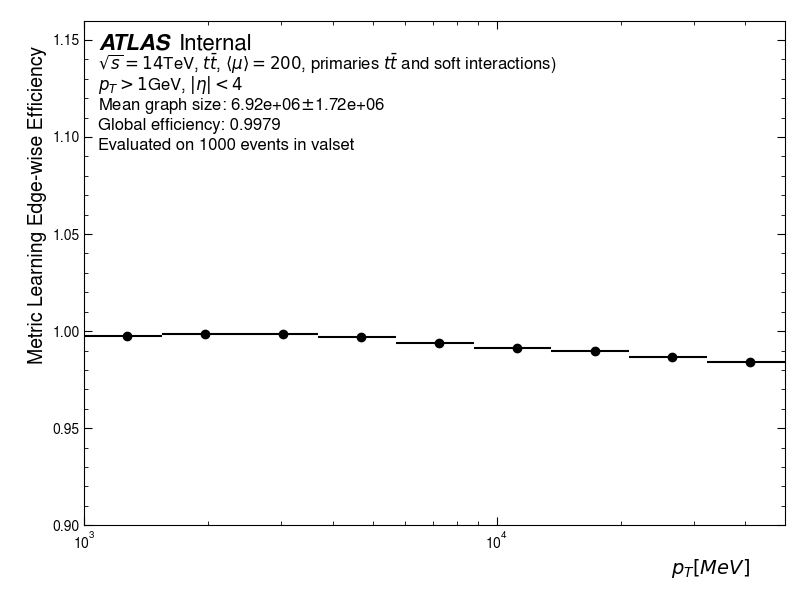
\includegraphics[width=\textwidth]{figures/metric_learning_eff_pt.png}
    \caption{}
    \label{subfig:metric-learning-eff-pt}
\end{subfigure}
\caption{Graph construction efficiency of the Metric learning approach as a function of $\eta$ (a) and $\pT$ (b), averaged over 1000 $t\bar{t}$ events. }
\label{fig:metric-learning-efficiency}
\end{figure}

The efficiency of graphs constructed with the Metric Learning method as a function of $\eta$ and $\pT$ is shown in figure \ref{fig:metric-learning-efficiency}. 
Good edge efficiency is observed across the $\eta$ range, averaging at $99.79\%$, on par with those from the Module Map under the \textbf{MinMax} selection, but with a considerably larger edge set, $\abs{V} = (6.92\pm 1.72)\times 10^6$, compared to just $(1.24\pm 0.36)\times 10^6$. 
As already discussed, the increased graph size will pose a problem for the edge-classifying GNN, so the graph is pruned using a light-weight neural network, which will be discussed in section \ref{sect:chap-gnn-filter-network}.
Although good efficiency is observed throughout the $\pT$ range, a slight decrease appears at $\pT>5$ GeV, which, similar to what that of the Module Map method, can be attributed to small training statistics at high $\pT$.
The metric learning model learns to minimize the distance between space points belonging to the same particle via an attractive term in the loss function (equation \eqref{eq:9.6}), which can be rewritten as
\begin{equation}
    \label{eq:9.8}
\mathcal{L}_{\theta} = E[d_\theta] =   \left( \sum_{\pT} E[d_{\theta} | \pT, \mathrm{target}] P[\pT|\mathrm{target}] P[\mathrm{target}] \right)  +  E[r-d_{\theta}|\mathrm{fake}] P[\mathrm{fake}],
\end{equation}
where $E[X]$ and $P[A]$ denote unconditional expectation value and probability, and $E[X|A]$ and $P[X|A]$ the conditional counterpart. 
The first term on the right-hand size, representing the attractive loss, is a sum over the $\pT$-dependant mean distance between nodes connected by a target edge, weighted by $P[\pT|\mathrm{target}]$, the probability that the edge comes from a particle having transverse momentum $\pT$.
As seen on figure \ref{subfig:pt-spectrum}, $P[\pT|\mathrm{target}]$ decreases monotonically with $\pT$, down-weighing the loss contribution, and thus directing the attention away from high-momentum particles.
As the curvature, which highly depends on $\pT$, is an important track pattern, the lack of high-$\pT$ examples impacts the performance of not only the metric learning, but also throughout the GNN4ITk algorithm.

